%In this section the available data sets must be presented. %The term dataset refers to any type of information source, for example web services for geolocation fall into this category. 
%In addition, all necessary data manipulation processes, such as cleaning and enrichment with external sources, must be presented and discussed.



Il Dataset consiste in un elenco di 1391082 prodotti descritti tramite le seguenti caratteristiche:
\subsubsection{Price}
\textbf{Price} rappresenta il prezzo per il quale l'articolo è stato venduto (variabile target).
Il prezzo medio è di circa \$26, con un valore minimo pari a \$0 e un valore massimo pari a \$2009; inoltre, presenta una deviazione standard di circa \$38.
Analizzando i percentili ci si accorge che i prezzi sono relativamente bassi in quanto il 75\% dei prodotti hanno un prezzo al di sotto di \$29.
\subsubsection{Train id}
\textbf{Train\_id} rappresenta l'identificativo del prodotto nell'elenco.
\subsubsection{Name}
\textbf{Name} è il nome del prodotto sotto forma di dato non strutturato.
\subsubsection{Shipping}
\textbf{Shipping} è caratterizzato dal valore 1 se la tassa di spedizione è a carico del venditore, altrimenti 0 se è a carico dell'acquirente.
Questo attributo è decentemente ripartito tra i venditori e gli acquirenti, in quanto il 55\% dei prodotti prevede un valore di 0.
Analizzando i prezzo degli articoli ci si aspetta che per quelli che la tassa di spedizione è a carico del venditore avranno un prezzo più alto. Tuttavia, ci sono una serie di fattori contrastanti. Questo può essere vero all'interno di specifiche categorie di prodotti e condizioni degli articoli, ma non quando si confrontano gli articoli sul totale. 
Infatti, il prezzo medio pagato dagli utenti che devono pagare le spese di spedizione (circa \$30) è superiore a quelli che non richiedono costi di spedizione aggiuntivi (circa \$22).
\subsubsection{Item condition}
\textbf{Item\_condition\_id} rappresenta lo stato del prodotto fornito dal venditore, questo valore varia da 1 a 5.
Il valore più frequente è 1, mentre 4 e 5 sono i più rari. Nei dati non è presente una descrizione dettagliata sul significato di questi valori, analizzando il dataset si può supporre che il valore 1 identifica la condizione migliore poichè è la più frequente, mentre il valore 5 identifica la condizione peggiore. Tuttavia calcolando i prezzi medi di vendita per ogni condizione non si riesce ad arrivare a una conclusione sicura poichè la condizione 5 è quella con il prezzo medio più alto, mentre la condizione 4 è quella con il prezzo medio più basso e le restanti categorie presentano un prezzo medio molto vicino.
\subsubsection{Category Name}
\textbf{Category\_name} rappresenta la categoria di prodotto a cui appartiene l'articolo.
Nel dataset sono presenti 1287 categorie univoche e tra ognuna di esse si vede una categoria principale/generale, seguita da due o più sottocategorie più specifiche (ad esempio: Women/Tops \& Blouses/T-Shirts). Inoltre, ci sono 6327 articoli che non hanno una categoria assegnata.
Infine, analizzando le dieci categorie più popolari, si nota che l'abbigliamento femminile è molto popolare su Mercari. Infatti, di queste prime dieci categorie 5 sono di abbigliamento femminile; Anche il trucco e l'elettronica sono categorie molto quotate.
\subsubsection{Brand Name}
\textbf{Brand\_name} rappresenta il marchio dell'articolo; nel dataset sono presenti 4809 valori differenti e 632682 valori mancanti.
\subsubsection{Item Description}
\textbf{Item\_description} rappresenta la descrizione del prodotto sotto forma di dato non strutturato. Nel dataset sono presenti 4 istanze senza descrizione e 82494 descrizioni con la stringa "no description yet".
Inoltre, non esiste una correlazione tra la lunghezza delle descrizioni e il prezzo, in quanto c'è una correlazione di 0.048.
Analizzando le word cloud ottenute tramite i bigrammi delle descrizioni  dei prodotti suddivisi in quattro fasce di prezzo: prezzo $>=$100 (Figura \ref{fig:100}), 50$<$ prezzo $<$100 (Figura \ref{Fig:50_100}), 30$<$ prezzo $<=$50 (Figura \ref{fig:30_50}) e prezzo $<=30$ (Figura \ref{Fig:minore_30}); si riescono a notare delle differenze sulle parole più frequenti. Infatti, nella wordcloud di Figura sono molto frequenti bigrammi che danno informazioni sulle buone condizioni dei prodotti, ad esempio:  100 authentic, great condition e good condition.
Diminuendo di prezzo questi bigrammi diventano meno frequenti, ma aumentano i bigrammi relativi a descrizioni mancanti.

\begin{figure}[H]
   \begin{minipage}{0.48\textwidth}
     \centering
     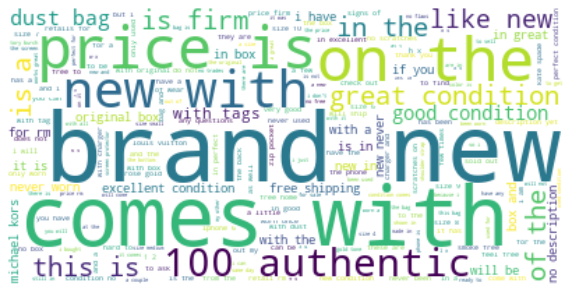
\includegraphics[width=.9\linewidth]{maggiore_100}
	\caption{Word Cloud contenente i bigrammi ottenuti dalle descrizioni dei prodotti con prezzo maggiore o uguale a 100}
	\label{fig:100}   
	\end{minipage}\hfill
   \begin{minipage}{0.48\textwidth}
     \centering
     
\includegraphics[width=.9\linewidth]{50_100}
     \caption{Word Cloud contenente i bigrammi ottenuti dalle descrizioni dei prodotti con prezzo maggiore di 50 e minore di 100}
     \label{Fig:50_100}
   \end{minipage}
\end{figure}

\begin{figure}[H]
   \begin{minipage}{0.48\textwidth}
     \centering
     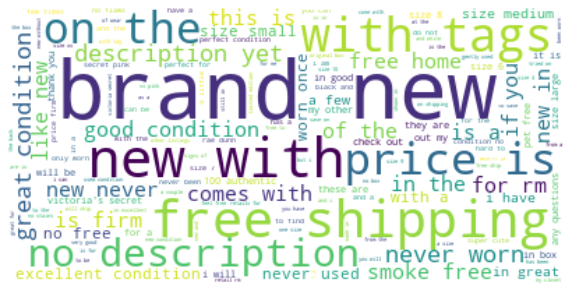
\includegraphics[width=.9\linewidth]{30_50}
	\caption{Word Cloud contenente i bigrammi ottenuti dalle descrizioni dei prodotti con prezzo maggiore di 30 e minore o uguale a 50}
	\label{fig:30_50}   
	\end{minipage}\hfill
   \begin{minipage}{0.48\textwidth}
     \centering
     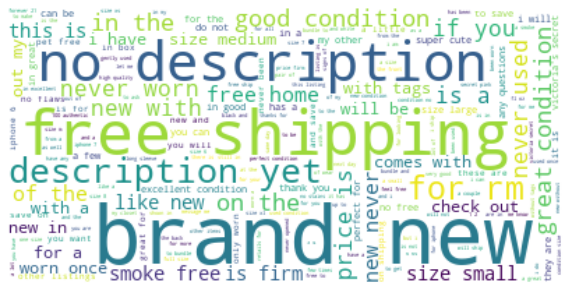
\includegraphics[width=.9\linewidth]{minore_30}
     \caption{Word Cloud contenente i bigrammi ottenuti dalle descrizioni dei prodotti con prezzo minore o uguale a 30}
     \label{Fig:minore_30}
   \end{minipage}
\end{figure}
\subsubsection{Pulizia Dataset}
Dal dataset sono stati eliminati tutti i prodotti con prezzi minori di cinque e maggiori di 2000 poichè sul sito ufficiale di Mercari è specificato che i prezzi possono essere impostati solo nell'intervallo [5,2000] (fonte: \url{https://www.mercari.com/us/help_center/article/69}).
Durante la fase di analisi si è scoperta la presenta di valori mancanti nei campi: item\_description, brand\_name e category\_name, questi valori sono stati rimpiazzati con il valore NA.
Inoltre, è stato effettuato un trattamento dei dati (cito paper sul text preprocessing) non strutturati convertendoli tutti in minuscolo, sono state sostituite le descrizioni mancanti con il valore NA (anche quando era presente la stringa "no description yet").
Sui dati testuali è stata effettuata una fase di lemmatizzazione (perchè usa vocabolario su cui tagliare le parole e cito articolo). Successivamente, sulle nuove parole ottenute è stata effettuata una fase di pulizia di questi campi non strutturati eliminando le stopwords, la punteggiatura, tutti i caratteri di lunghezza pari a 1 che non sono numeri (è stato deciso di mantenere tutti i numeri poichè molte descrizioni senza di essi perdono di significato) e sono state eliminate le emoji.


I valori del campo category\_name sono stati codificati in interi tramite la tecnica label ecoding.
\end{document}


